\subsection{Structures (\textit{CE})}
\subsubsection{Material Selection (\textit{CE})}
Modern-age aircraft exhibit many different structure layouts and material selection for each structure. The goal for the material selection is to meet the given requirements, as well as provide an aircraft which will have the best mechanical properties for the given flight missions. The different structure types are tabulated in Table \ref{tab:structure_material_table}.

\begin{table}[!h]
\centering
\caption{Structures Build-up Descriptions }
\label{tab:structure_material_table}
\begin{tabular}{ |p{2cm}||p{13cm}| }
\toprule
\multicolumn{1}{|c||}{\textbf{Build-up Type}} & \multicolumn{1}{c|}{\textbf{Description}}                                                                                                                       \\ \hline\hline
Metal                                       & Most or all parts of the primary and secondary structure are metallic, such as aluminum, steel, and titanium alloys                                             \\ \hline
Composite                                    & Most or all parts of the primary and secondary structure are composite, such as carbon fiber reinforced polymers (CFRP), fiber glass, or other composites \\ \hline
Hybrid                                       & Depending on the structure, the material of the structure is either metal or composite                                                                            \\ \bottomrule
\end{tabular}
\end{table}
% \begin{tabular}{ |p{3cm}||p{3cm}|p{3cm}|p{1.5cm}|p{3cm}| }

Metallic build-up is the more traditional method of designing aircraft structures, where most or all primary structures are composed of metal alloys. This method of construction is typically cost-effective and weight efficient for most structures, however, there are downsides such as damage tolerance and fatigue. A composite build-up requires high development costs, and relatively high manufacturing costs, but can offer incredible weight-savings compared to metal structure due to their high strength-to-weight ratio. In Figure \ref{fig:strength_density}, the ultimate tensile strength versus the density of the material can be seen for many different categories of materials \cite{ashby}. Note that composites have a higher strength to weight ratio that most metal alloys. 

\begin{figure}[!h]
    \centering
    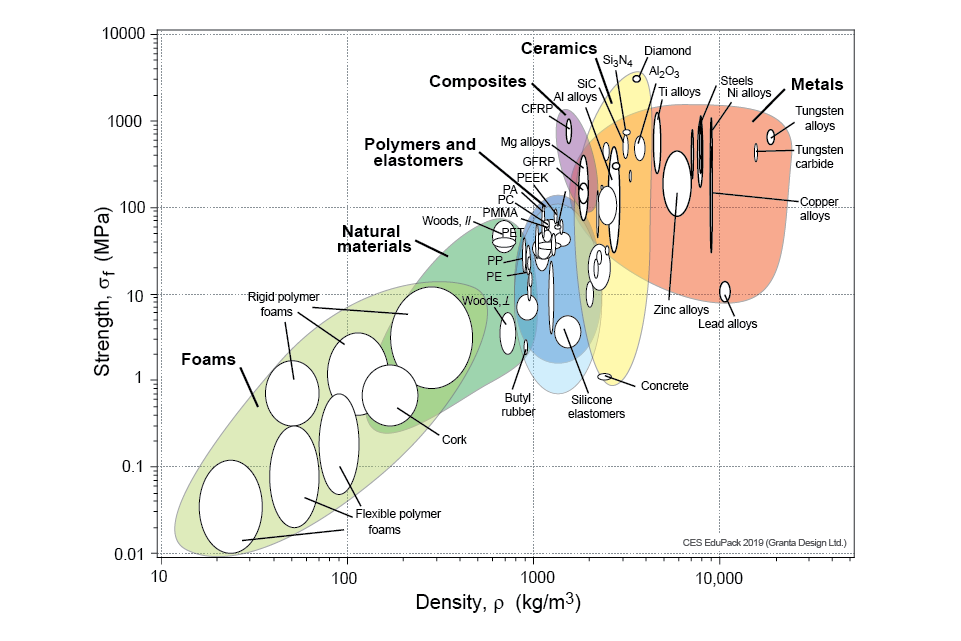
\includegraphics[width=\linewidth]{Photos/strength_density.png}
    \caption{Strength versus Density for Different Materials}
    \label{fig:strength_density}
\end{figure}

A hybrid build-up is a method where both metals and composites are used for different structures depending on key factors such as fatigue, damage tolerance, ultimate strength per density ratio, cost of manufacturing, assembly methods, and operational costs. Hybrid designs usually optimized costs and weight of the structure, which results in the wings and stabilizers to be a mainly composite build-up, and the fuselage and other secondary structures to be a metal build-up. Hybrid construction is a newer technology, and as the development of manufacturing of composites advances, this style of construction may become more prevalent in industry. A notable aircraft which uses a hybrid build would be the Boeing 777-X, in which the wings and stabilizers are composite and the fuselage is metallic. The reason the fuselage is metallic and not composite comes down to the difficulties in manufacturing a round and continuous composite structure, such as the fuselage and empennage sections. A notable aircraft which utilizes mainly composite construction is the Boeing 787, as seen in Figure \ref{fig:787 materials} \cite{787_Mat}.

\begin{figure}[!h]
    \centering
    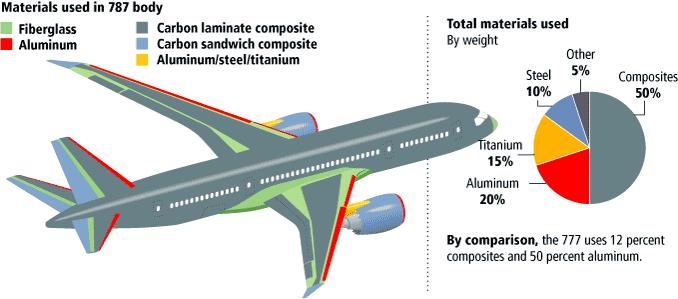
\includegraphics[width=\linewidth]{Photos/787 Materials.png}
    \caption{Material Composition of the B787}
    \label{fig:787 materials}
\end{figure}

\FloatBarrier
In Table \ref{tab:pugh_structures}, the benefits and costs for each build-up construction method were weighed in a Pugh matrix given the requirements of cost reduction and the desired aspect ratio and wingspan.

\begin{table}[!h]
\centering
\caption{Pugh Matrix for Structures Material Selection}
\begin{tabular}{|p{3.5cm}||p{2cm}|p{2cm}|p{2cm}|p{2cm}| }
\toprule
\multicolumn{1}{|c||}{\textbf{Criteria}} & \multicolumn{1}{c|}{\textbf{Weight}} &  
\multicolumn{1}{c|}{\textbf{Metallic}} & \multicolumn{1}{c|}{\textbf{Composite}} & \multicolumn{1}{c|}{\textbf{Hybrid}} \\ \hline \hline 
Cost & 10 & 9 & 7 & 8 \\ \hline
Manufacturability & 8 & 8 & 5 & 7 \\  \hline
Strength to Weight & 8 & 7 & 8 & 9 \\  \hline
Fatigue Rating & 5 & 6 & 8 & 7 \\  \hline
Damage Tolerance & 5 & 7 & 6 & 7 \\  \hline
Corrosion Resistance & 4 & 4 & 9 & 8 \\  \hline
Environmental Impact & 3 & 8 & 4 & 6 \\  \hline \hline
 & \textbf{Total} & \textbf{315} & \textbf{292} & \textbf{328} \\
\bottomrule
\end{tabular}
\label{tab:pugh_structures}
\end{table}
\FloatBarrier

Given the Pugh matrix, a hybrid construction is most ideal for the given aircraft requirements. A low fidelity analysis of the structure can assume an isotropic material with the mechanical properties of an ideal composite layup to create a factor to apply to estimations of structure loading given by Raymer \cite{raymer}. A high fidelity analysis of the composite structure would require one of two methods: run FEA on an isotropic material with similar properties to an ideal composite layup, or run FEA with a specific composite build-up in a capable software such as ANSYS.

\subsubsection{Construction and Layout (\textit{CE})}
Given the hybrid construction method, the wings and stabilizers require a newer method of construction compared to the traditional metallic construction. Since composite layups are essentially an additive manufacturing technique, the stringers can be integrated into the upper and lower panels of the wings and stabilizers. This alone saves incredible costs and weight by eliminating the use of fasteners in high-load locations. The absence of fasteners increases the damage tolerance and fatigue rating of the structure as well.

Spars are the most important structure to the wings, and arguably the most important on the entire aircraft. These few parts make the entire aircraft fly, and in the process, see a lot of loading cycles over the life of the aircraft. In metal structures, loading cycles cause fatiguing, and then fatigue cracking, which degrades the structure. Traditionally, metallic structures use a 3-piece build-up for the spar: chord on the top and bottom, and a web connecting the two chords. This structure ends-up looking like a C-channel extrusion. The reason the spars are a 3-piece build-up comes down to crack growth and fatigue. A crack starts in the lower chord, but cannot grow through the entire spar since the chord is connected to the web by fasteners. There are a few aircraft that have used a one-piece, or monolithic, metallic spar, some being the Boeing 1-B and the Airbus 320 NEO. There is significant research in learning crack-growth patterns and predicting where cracks will start and grow; opening-up huge possibilities in reducing manufacturing costs by allowing optimized metallic spars to be utilized on low-cost aircraft.

\newpage
The spars are where composites differ greatly from traditional 3-piece spar construction. Since composite structures do not crack like metal structures when fatigued, a monolithic spar can be utilized. This spar construction reduces costs, but increases the weight due to a thicker layup compared to a simpler 3-piece construction. Due to the considerable cost savings, a monolithic composite spar was modelled, seen in Fig. \ref{fig:spar_layout}.

\begin{figure}[!h]
    \centering
    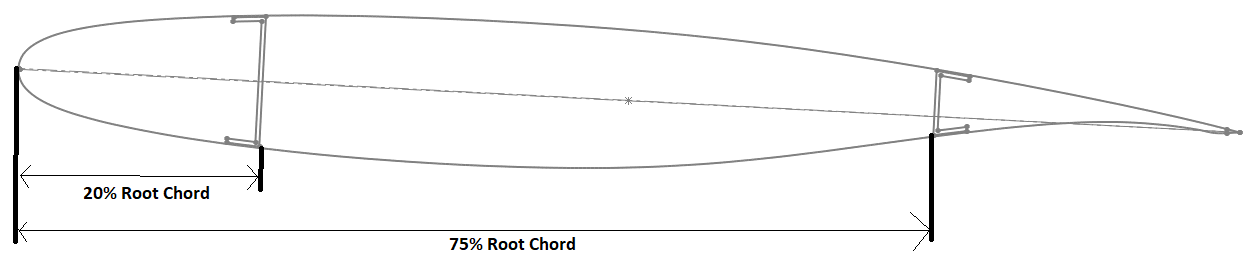
\includegraphics[width=\linewidth]{Photos/structuresandloads/Spar Layout.PNG}
    \caption{SAM Mk. I Spar Cross Section at the Root Chord}
    \label{fig:spar_layout}
\end{figure}

Ribs in the wings are traditionally multi-piece substructures comprised of machined aluminum parts. The benefit to using aluminum ribs in the wing comes from the fact that composites are difficult to utilize on very complex and dramatic geometry. However, due to manufacturing costs, a multi-piece composite rib was chosen over a monolithic metallic rib. In an effort to save more cost and manufacturing troubles, a monolithic rib structure, with the rib posts, chords, webs, and pads formed in a single composite part, can be investigated at a later date. Ribs in the stabilizers are typically not as complex as a rib in the wings due to the lower-loaded and smaller structure. In the stabilizers, composite ribs may be utilized for weight savings. The current rib spacing is \~30 inches, which is a derivative of the approximation given by Raymer with a slight adjustment for composite composition. A more detailed analysis is needed to improve spacing and sizing of the ribs \cite{raymer}.

Since the fuselage is a metallic structure, a common layout of frames, stringers, and floor joists can be utilized. The floor joists may be a composite part, as the joists are not primary structure, and the connection method to the frames of the fuselage is by brackets and fasteners. Frames in the business class are spaced with the same distance of the business class seat pitch, and the economy frames are spaced the same distance of the economy seat pitch. The seat pitches are defined in Section \ref{section: internal config}. The frames and stringers are spaced such that no windows or exit doors are covered or physically blocked. Several frames will be considered "floating", or not connected to the skin of the fuselage, and others being traditional frames. The floating frames are only mounted to the stringers, rather than the actual skin of the fuselage. Floating frames increase fatigue life, as fewer holes are introduced into the fuselage skin. It will also need to be noted that frames cannot be present where emergency exit doors and windows exist.

In Fig. \ref{fig:structure_cutaway}, the aircraft structure can be seen. It should be noticed that no windows or doors are covered by frames or stringers in the fuselage. Also note that at this time, the nose ribs have not been modelled, as their current spacing and size is not fully defined at this time.

\begin{figure}[!h]
    \centering
    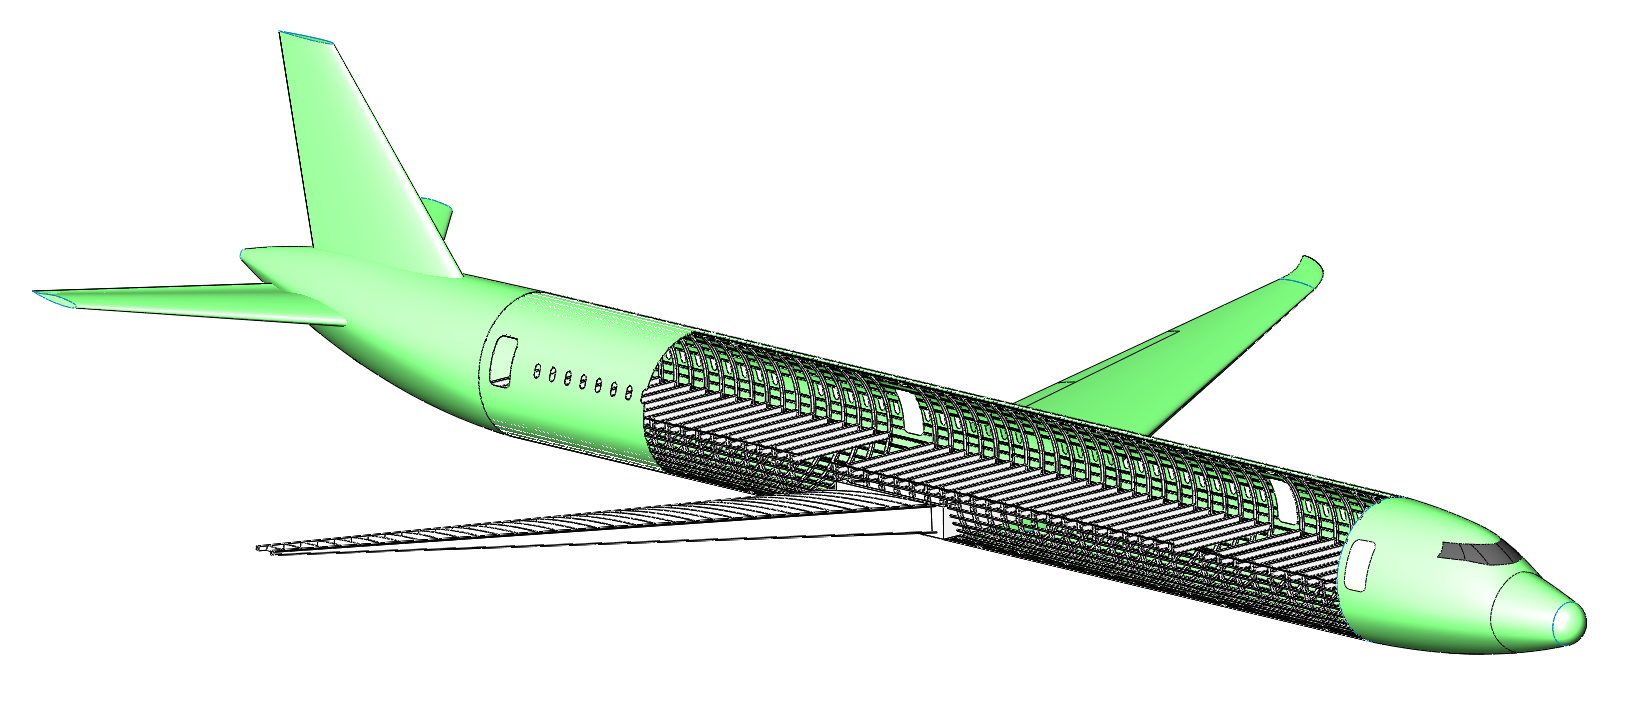
\includegraphics[width=\linewidth]{Photos/structuresandloads/Updated Sctructures Cutaway.PNG}
    \caption{SAM Mk. I Structures Model Cutaway}
    \label{fig:structure_cutaway}
\end{figure}

\subsubsection{Wing Attachment and Configuration}
There are two primary methods of mating the wings and the fuselage: "bolt-on" and "drop-in". These methods are both commonly used in industry, as both offer different advantages and carry their own disadvantages. 

A "bolt-on" method essentially bolts the wings onto the fuselage through the wingbox, as the wingbox is integrated into the fuselage. Utilizing shear plates or tension bolts, each wing is attached to the fuselage using fasteners. This method is preferred by most aircraft manufactures, as manufacturing of the fuselage with an integral wingbox and two separate wings is easier to manage in an assembly line in most cases. Using fasteners to attach the wing to the fuselage from the outside poses a difficult engineering challenge which is to make sure load paths are correctly transferring load to the correct primary structures.

The "drop-in" method refers to dropping the fuselage into the space made by the wingbox and wing superstructure. In this method, the wings and wingbox are a singular structure, and the fuselage does not have an integral wingbox. Due to the wings and wingbox being connected before the mating to the fuselage, a more robust connection to the wingbox (internal connection of the spars to the wingbox, rather than fasteners) can be achieved. 

Given that the aircraft is a wide-body, large wingspan structure, a bolt-on method would be preferred, as the manufacturing and logistical challenges in a "drop-in" method are costly. Choosing to use the bolt-on method, the wing was then designed accordingly. In Fig. \ref{fig:wing_structure}, the wing and wingbox structure can be seen.

\begin{figure}[!h]
    \centering
    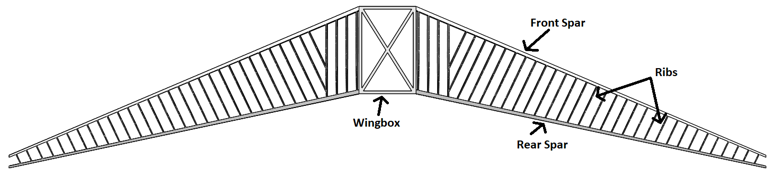
\includegraphics[width=\linewidth]{Photos/structuresandloads/Wing Structure.PNG}
    \caption{SAM Mk. I Wing Structure Top View}
    \label{fig:wing_structure}
\end{figure}
\FloatBarrier

It can also be seen in Fig. \ref{fig:wing_structure} that the ribs of the wing are currently modelled such that they are parallel to the stream-wise direction. Typically this is unconventional, as stress risers form at the rib and spar junction (at the rib posts). A more structurally sound and easy to manufacture configuration would be to align the ribs to be perpendicular to the quarter-chord or front spar.

\subsubsection{Future Work for Structures (\textit{CE})}
Future work includes several key tasks. First item to tackle is carrying-out a full FEA analysis on the wing and fuselage. In the CAD model, the structure of the aircraft needs to be improved by adding more detail to the stabilizers and the nose cone once geometric sizing is completed, as well as change the direction of the ribs to be perpendicular to the quarter-chord or front spar to minimize costs and stress risers. Some more future work includes the creation of useful trade studies, particularly trade studies comparing the sizing of the spars and spacing of the ribs in the wing to the stiffness and weight of the wing. 

\subsection{Loads (\textit{MK})}
\subsubsection{V-n Diagram}
\label{subvn}
One important aspect in the structural analysis of the aircraft is determining the limits in the performance of the aircraft. This is done using a V-n diagram, as shown in Figure \ref{figVN}. This diagram incorporates parameters such as wing loading and performance velocities (maneuvering, cruise, and dive velocities) along with limit loading factors. Maximum positive and negative limit loading factors of 2.15 and -1.0 were chosen, respectively, according to the regulations set forth in FAA 14 CFR Part 25.337 \cite{cfr}, Limit Maneuvering Load Factors. Additionally, gust loads were added according to CFR Part 25.341 \cite{cfr}. The gust load lines were further calculated using a safety factor of 1.5, as specified in FAA 14 CFR Part 25.303, Factor of Safety \cite{cfr}. Note that the velocities displayed in the diagram (Figure \ref{figVN}) units displayed as equivalent velocities (KEAS). This V-n diagram was created assuming sea-level conditions. 

\begin{figure}[H]
    \centering
    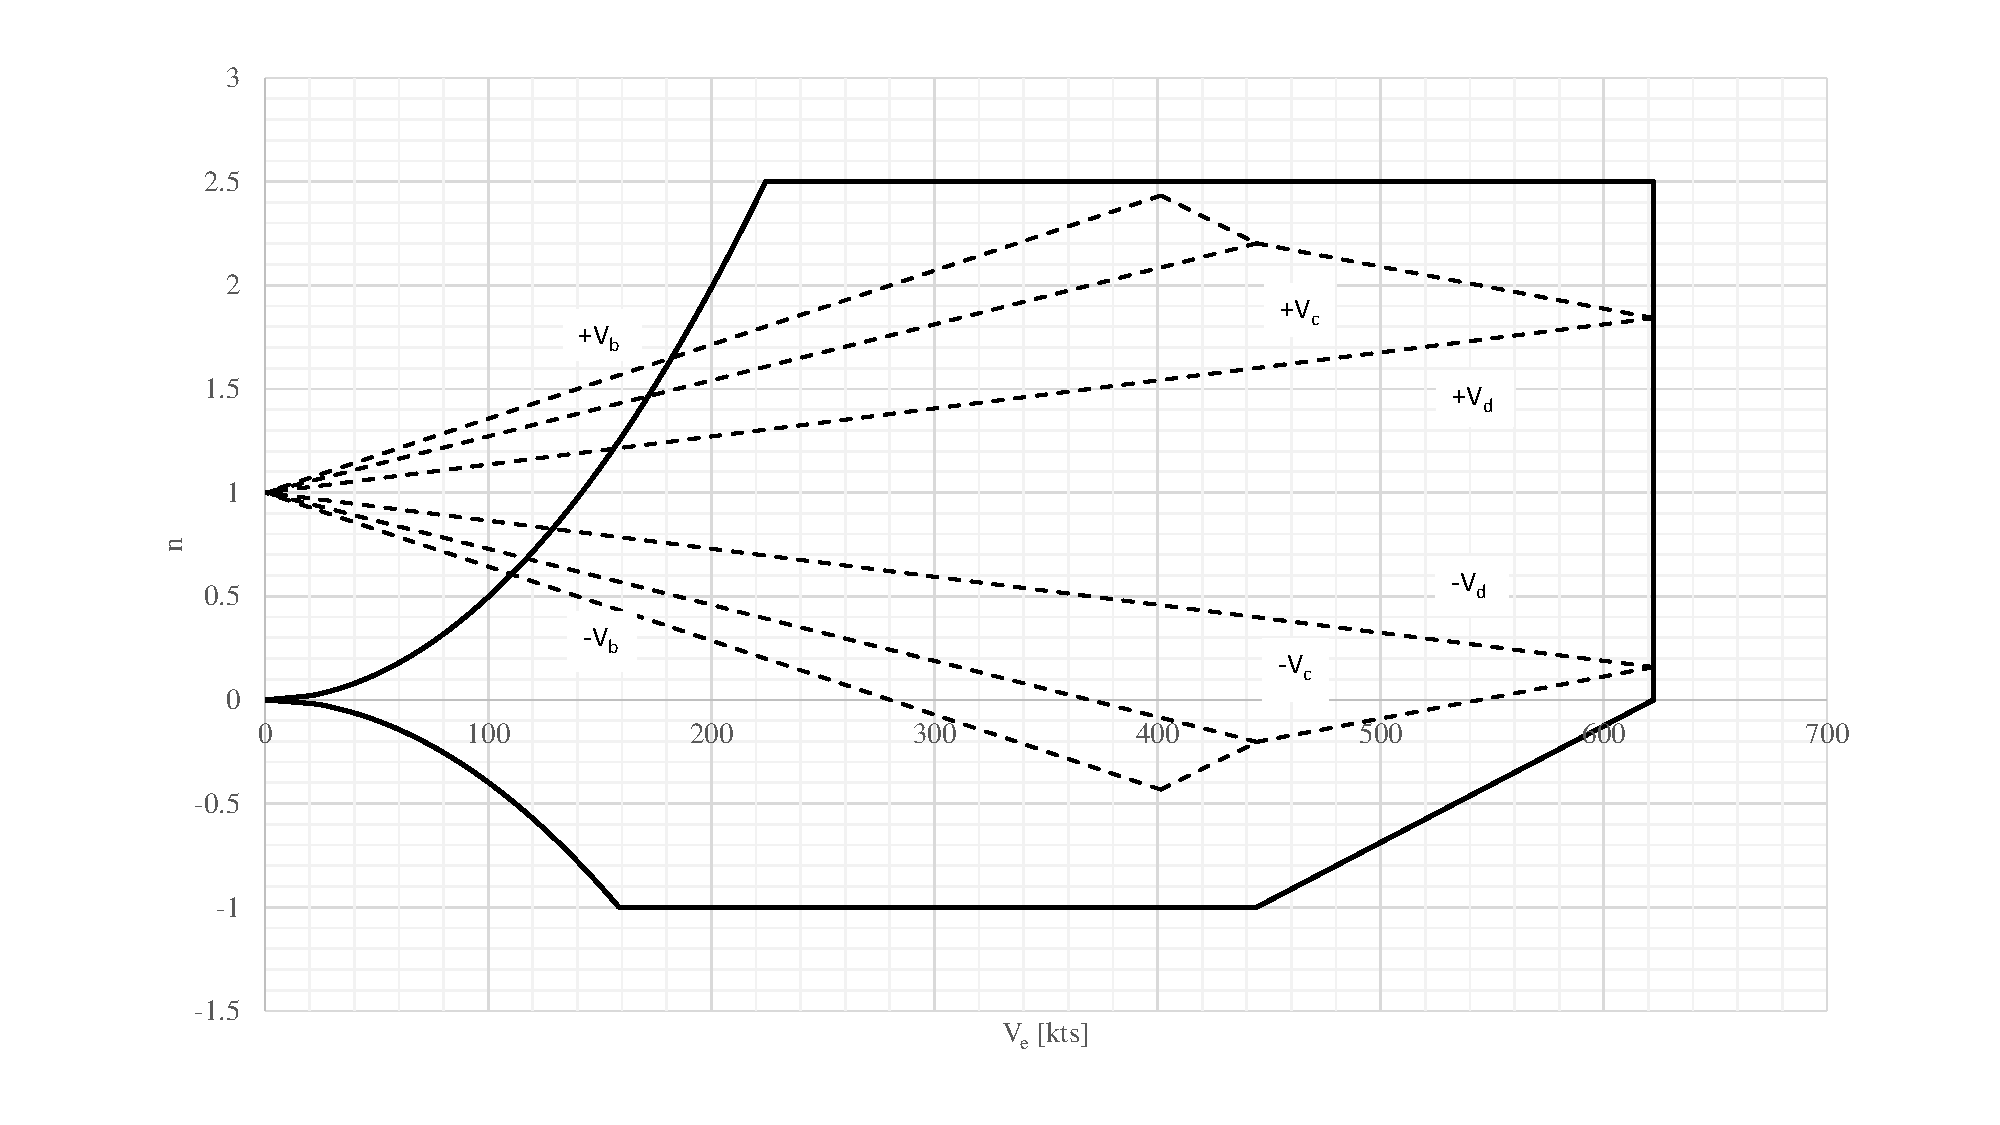
\includegraphics[width=\linewidth]{Photos/VN_Diagram.pdf}
    \caption{V-n Diagram of Limit Load Factors}
    \label{figVN}
\end{figure}

Using equations from Roskam \cite{roskam_5}, design maneuvering speed ($V_{A}$), cruising speed ($V_{C}$) and design diving speed ($V_{D}$) were estimated to be 208 kts., 422 kts. and 527 kts, respectively. Furthermore, the calculation of the positive and negative stall lines involved the use of equations from Roskam \cite{roskam_5}. At sea-level and at a limit loading factor of 1 and -1, the stall speeds were calculated to be 142 kts. and 159 kts., respectively.

\subsubsection{Wing Loading}
\label{winlod}
The loading experienced on the wing was analyzed. Specifically, Schrenk's approximation was used to estimate the span-wise loading on the wing, using equations found in Chapter 14 of Raymer \cite{raymer} as well as the positive limit loading factor from the V-n Diagram. First, the elliptical loading was estimated across the wing. Then, a rectangular method was used to estimate the loading on the wing. Both of these methods required the Schrenk's Approximation Set, which was estimated to be about 726,360 lbf. Then, Schrenk's approximation takes the average of the elliptical distribution and a rectangular distribution to provide a semi-empirical approach to visualizing the load distribution on the wing. Figure \ref{schrenk} shows the wing loading using Schrenk's approximation along with the elliptical and rectangular approximation across half the wing, with the other half being symmetric. 

\begin{figure}[H]
    \centering
    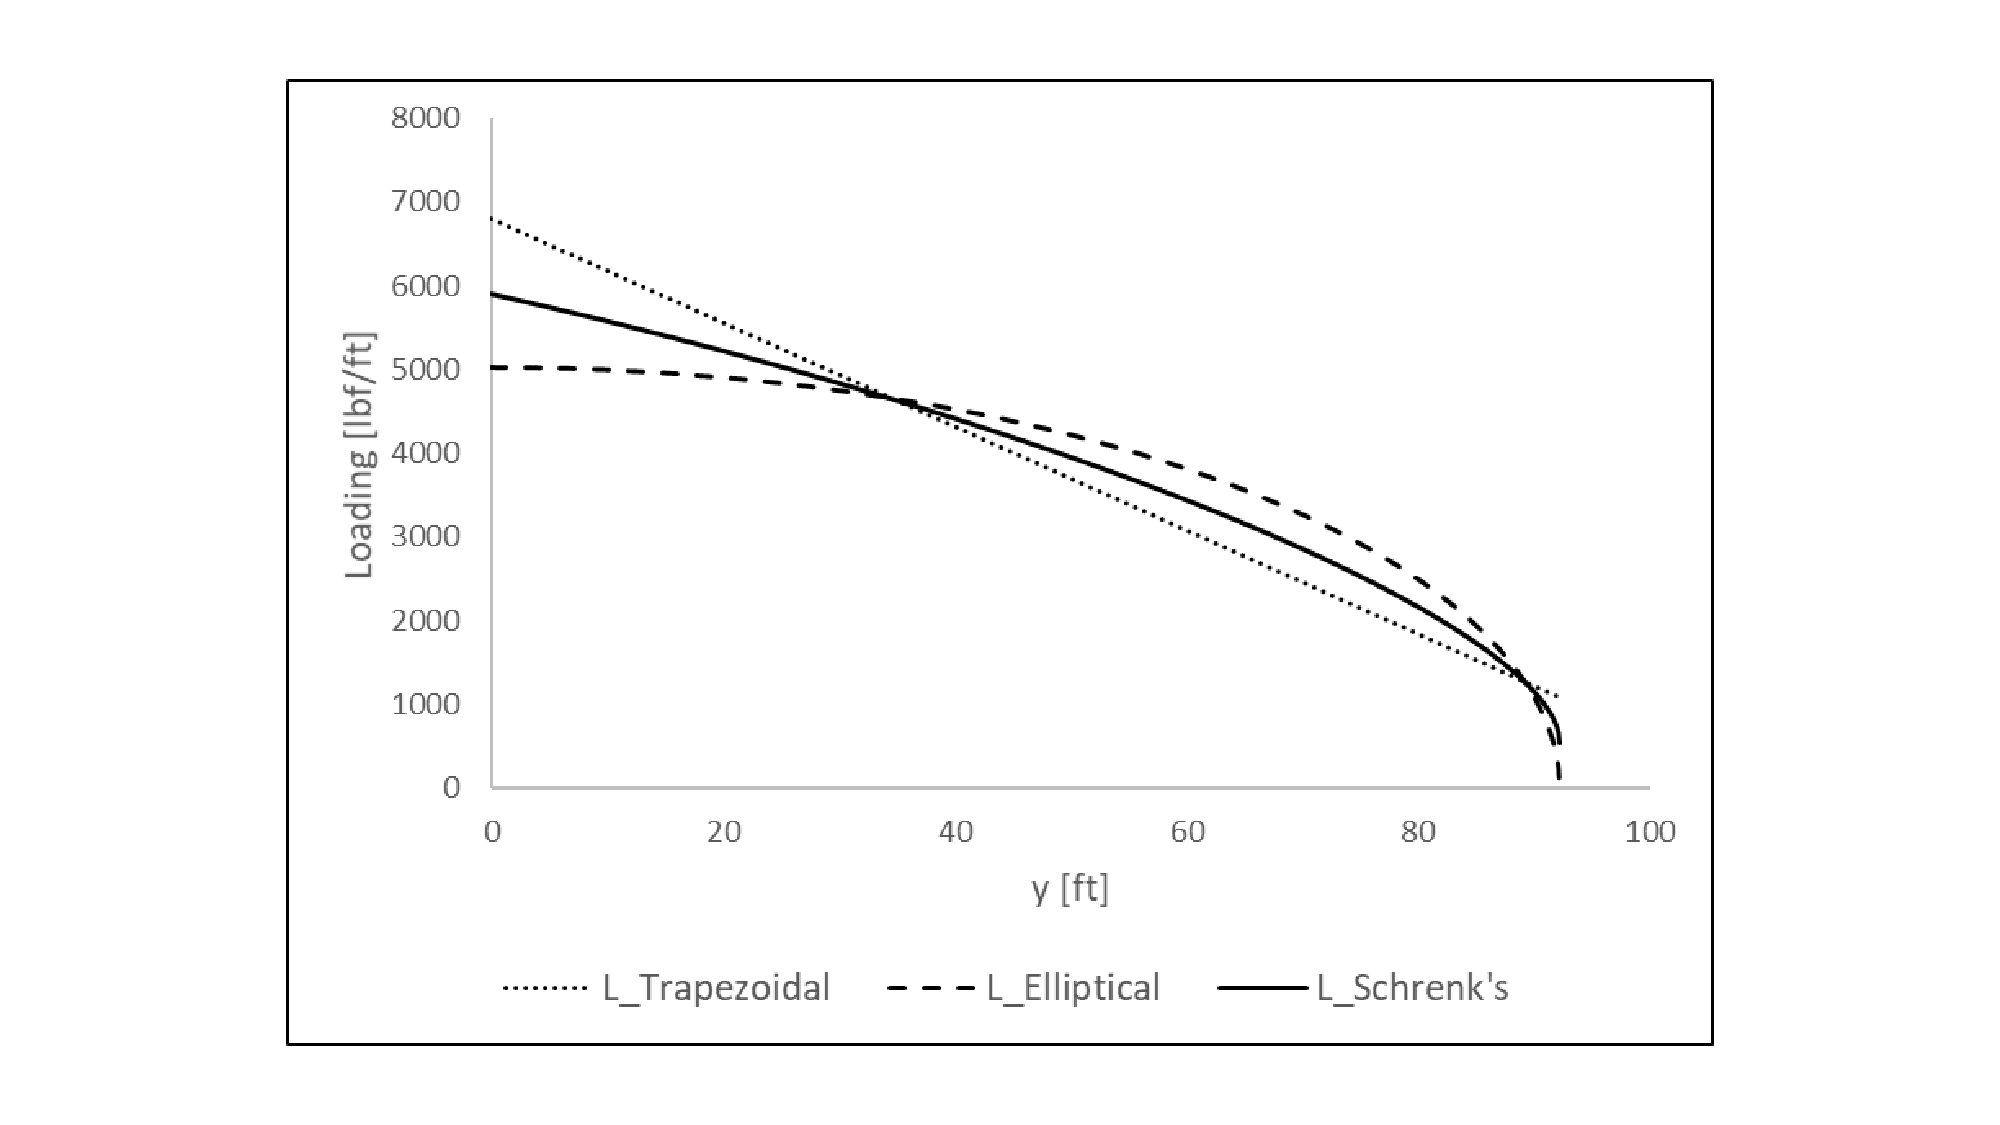
\includegraphics[width=1.0\linewidth]{Photos/Loading.pdf}
    \caption{Load Distribution Across the Half-span Wing}
    \label{schrenk}
\end{figure}

After estimating the load distribution on the wing, the internal forces of the wing are to be determined. Team Toucans implemented a numerical integration scheme, in which the Schrenk's diagram was integrated to obtain a shear diagram. This shear diagram was then integrated again to derive the bending moment diagram. The integration method of choice was the trapezoidal method. Both of these diagrams are modeled on the half-span of the wing, thereby assuming symmetry. Figures \ref{sheardiag} and \ref{momentdiag} show the Shear and Bending Moment diagrams as functions of half the span of the wing, respectively. Note that the shear loading and bending moments are zero at the tips and maximum at the center of the wing. 

\begin{figure}[H]
    \centering
    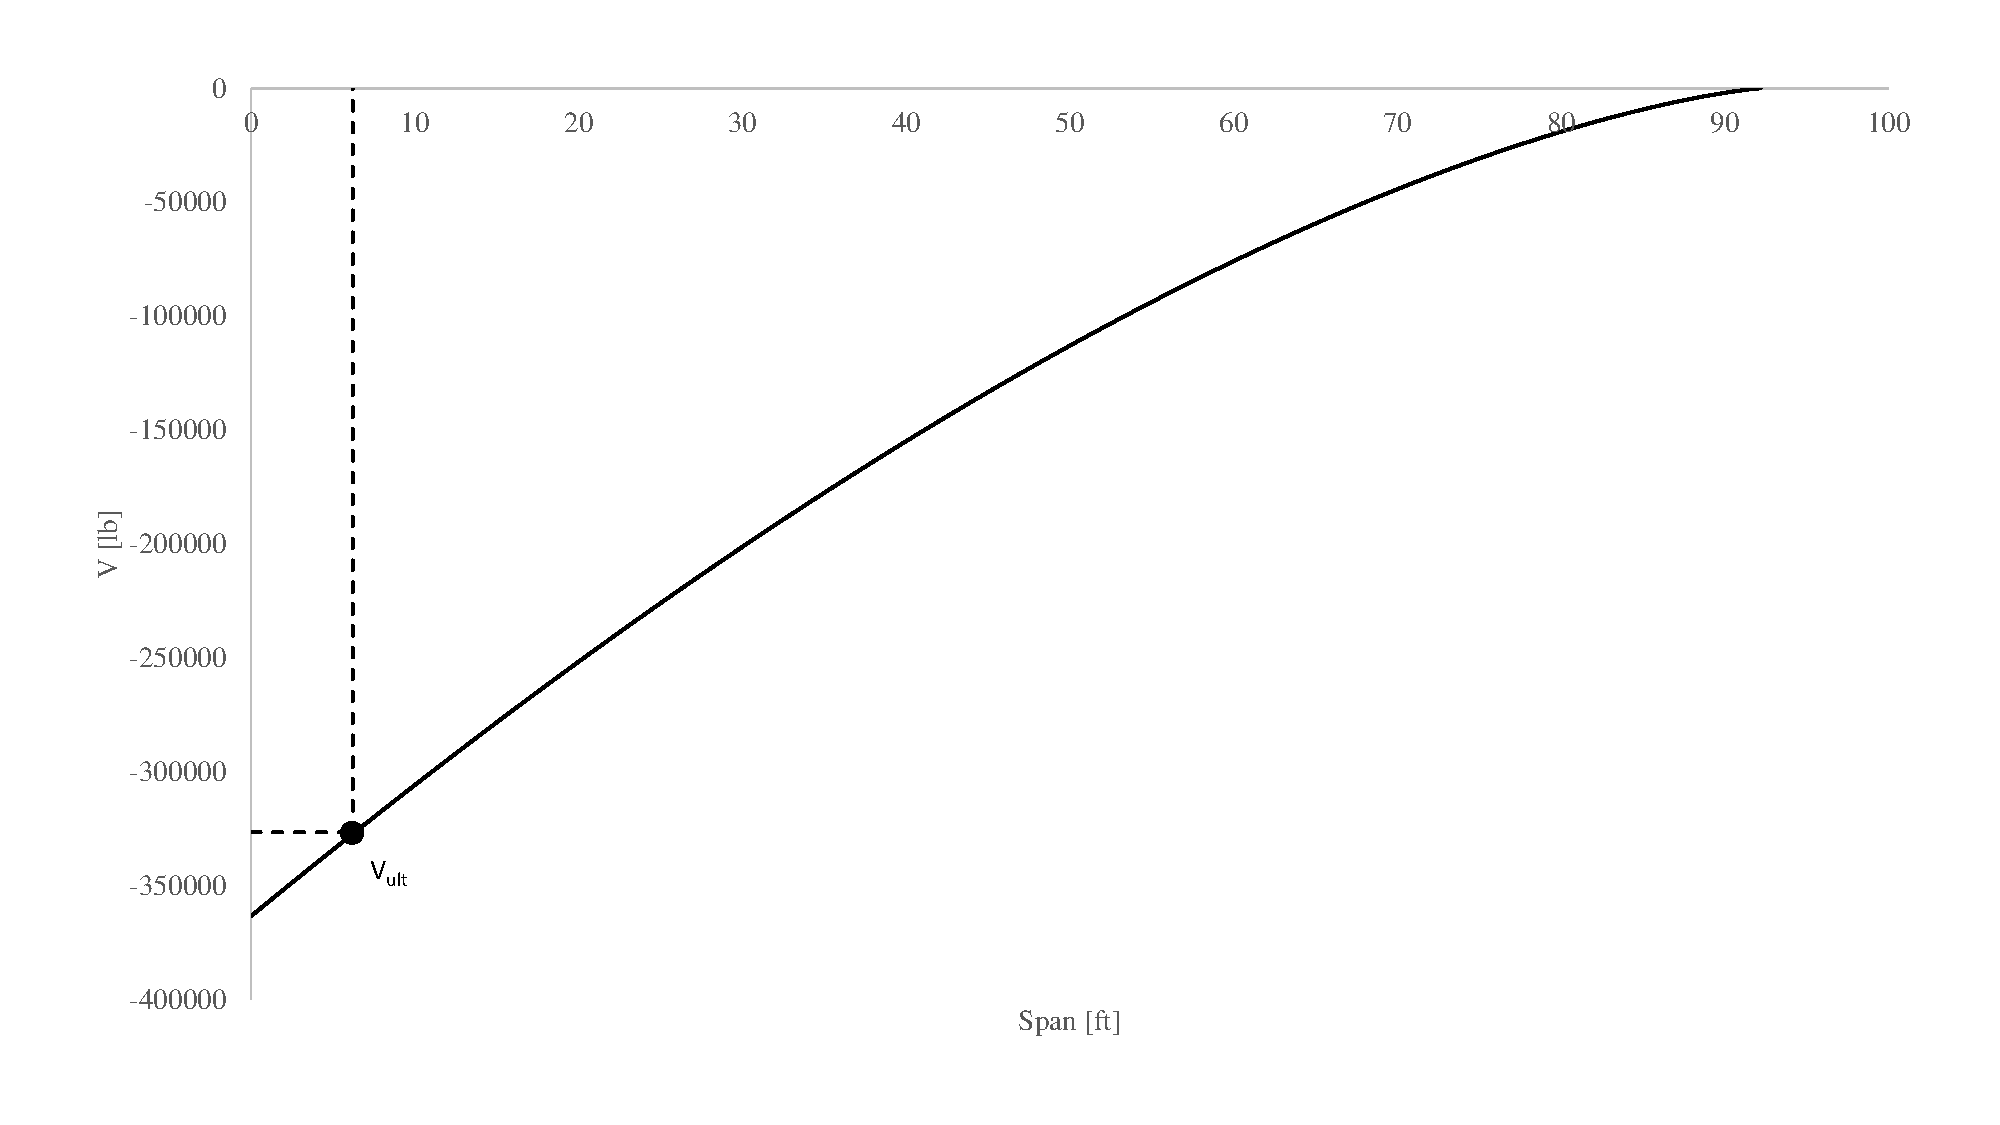
\includegraphics[width=1.0\linewidth]{Photos/Shear.pdf}
    \caption{Shear Diagram Across the Half-span Wing}
    \label{sheardiag}
\end{figure}

\begin{figure}[H]
    \centering
    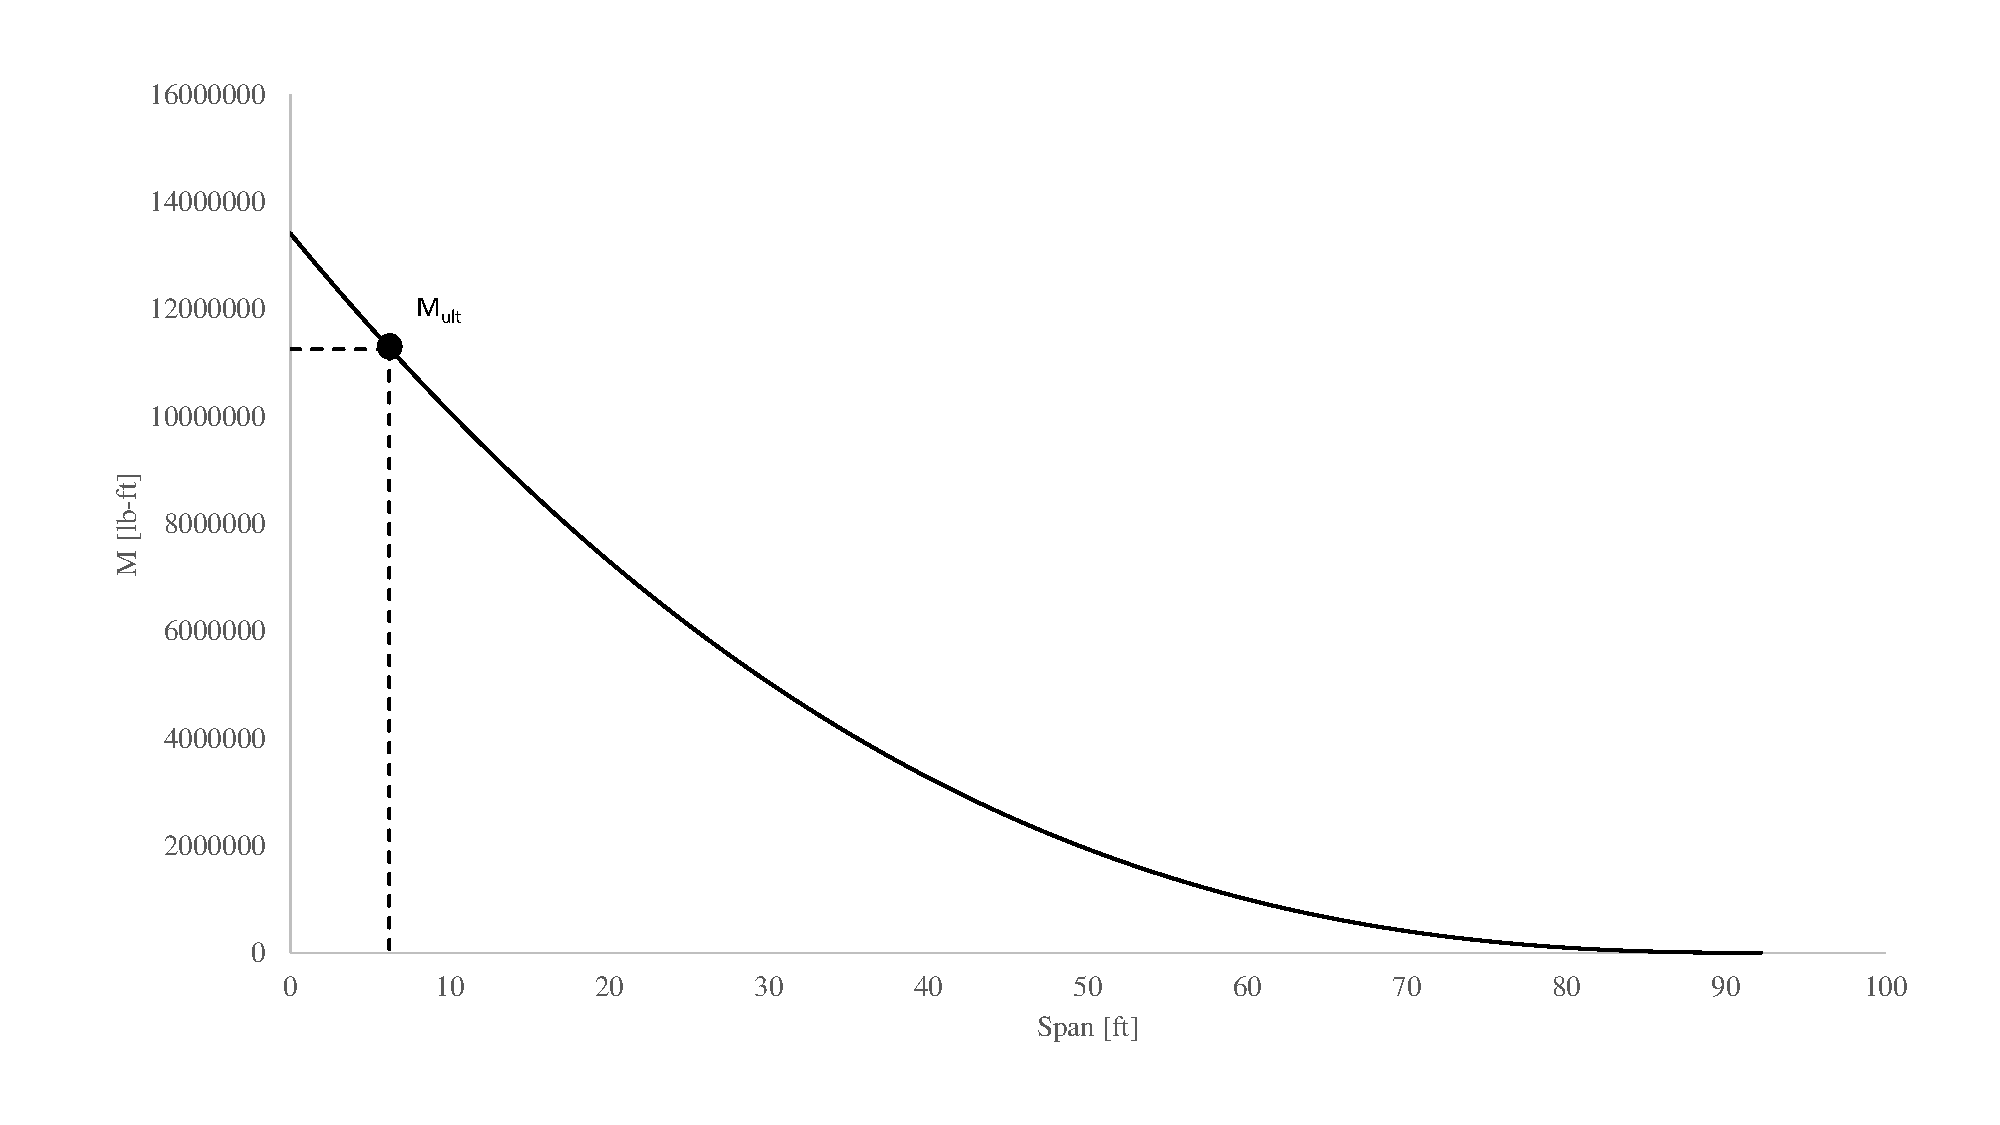
\includegraphics[width=1.0\linewidth]{Photos/Moment.pdf}
    \caption{Bending Moment Diagram Across the Half-span Wing}
    \label{momentdiag}
\end{figure}
\clearpage
Finally, the ultimate shear load and ultimate bending moment need to be determined. These can be estimated by estimating the distance from the center of the fuselage to the location of the wing attachment to the fuselage. This wing attachment location was estimated to be 6.2 ft from the center of the fuselage. This location is where the wing will feel the ultimate shear load and bending moment, which were estimated to be -326,600 lbf and 11,251,000 lbf-ft, respectively. These are represented in Figures \ref{sheardiag} and \ref{momentdiag} as red dots. 

\subsubsection{Load Paths}
As the wing is experiencing aerodynamic loads, those loads are transferred onto the structure of the aircraft. From the Schrenk's approximation of the lift distribution across the wing, the load then gets transferred onto the wing panels. From there, the loading transfers onto the spars, which lead to the wing box. Then, from the wing box, the loading goes into the fuselage, where the maximum loading occurs. The ribs on the wing absorb the shear produced by the bending moment from the lift distribution. Additionally, the engine also produces a load onto the wing. This loading follows a similar path, except it moves into the pylon first, then into the wing panels. From there, the load transfers into the spars, which moves into the wing box, and finally into the fuselage. Figure \ref{loadpath} shows a diagram of the load paths across half the aircraft, since it will be symmetric along the center line of the fuselage. 

\begin{figure}[H]
    \centering
    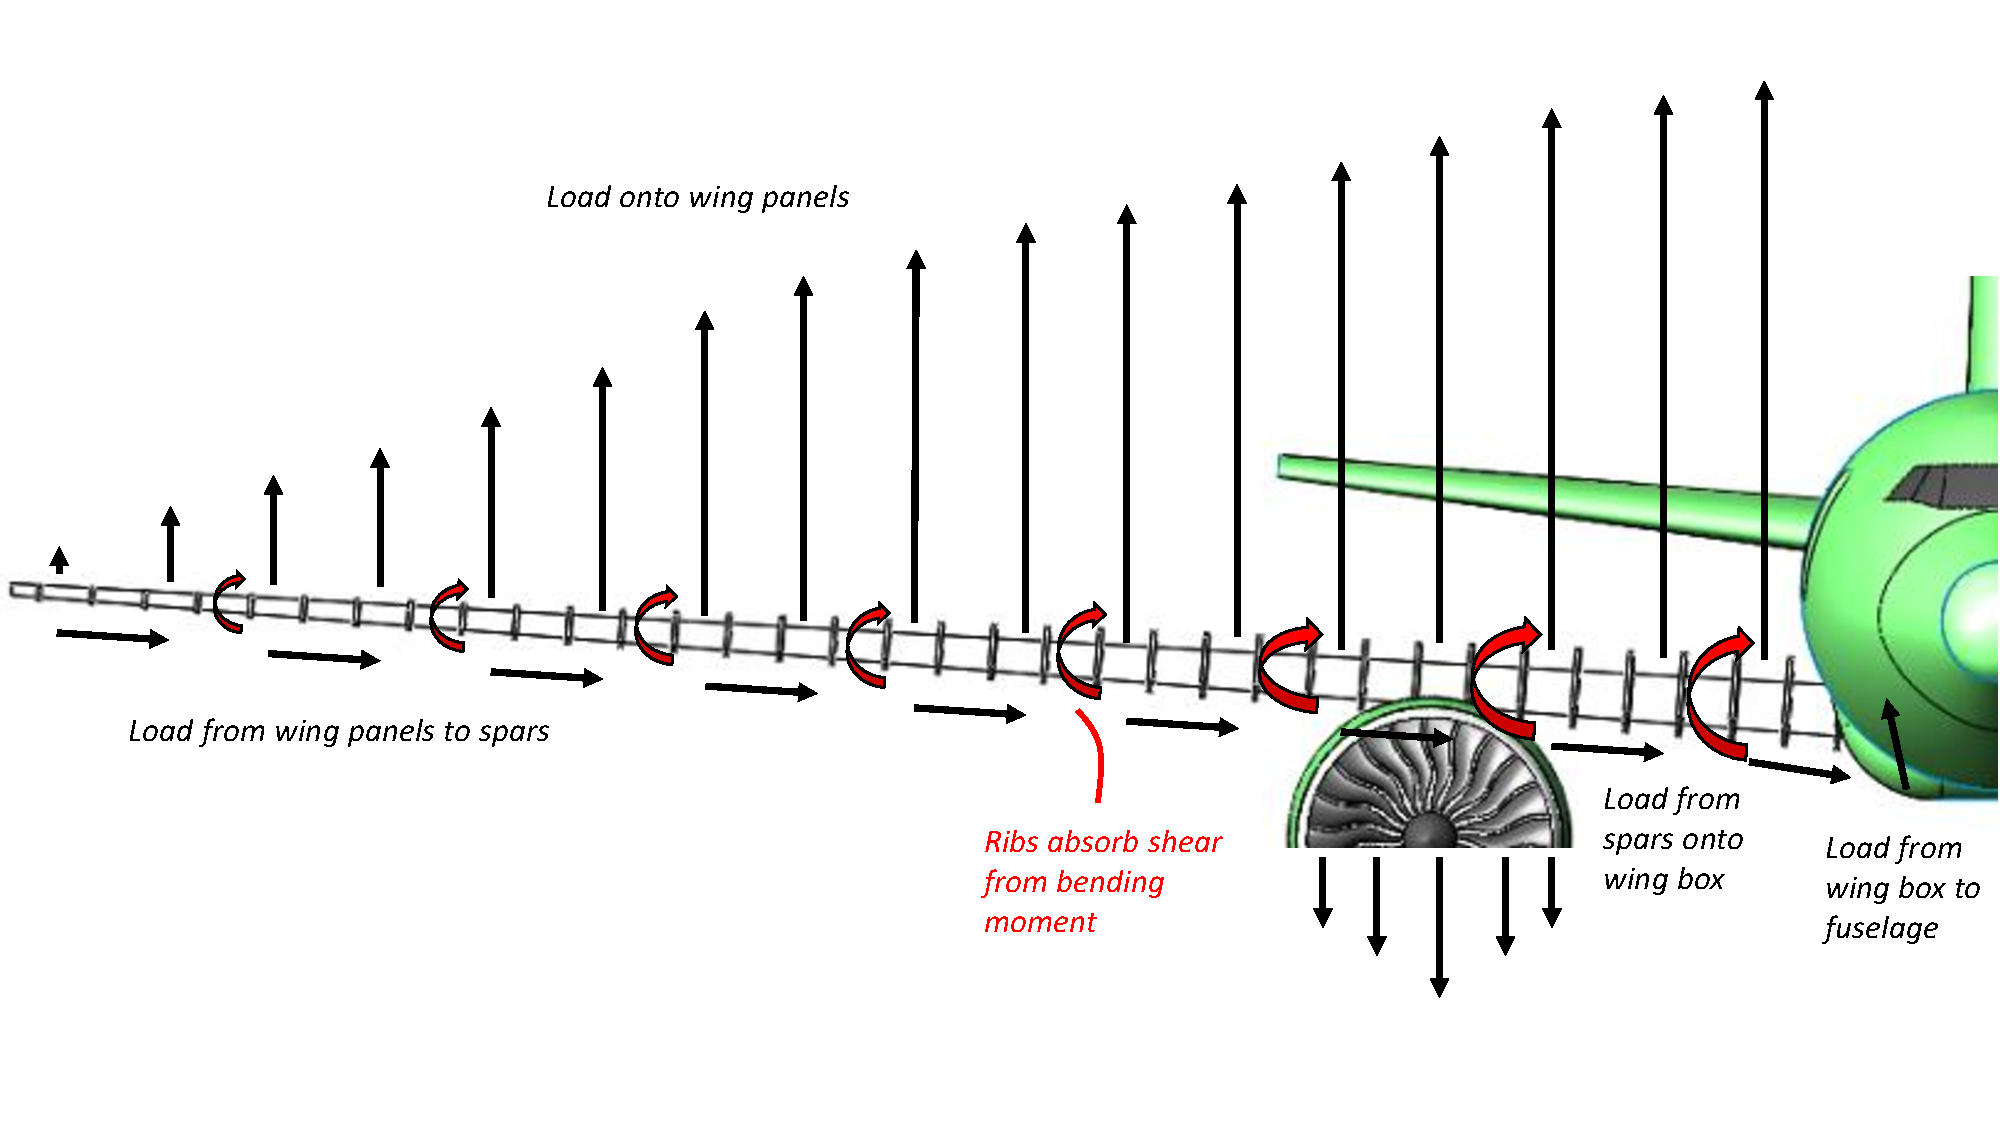
\includegraphics[width=1.0\linewidth]{Photos/Load_Path.pdf}
    \caption{Load Path of the Lift Distribution and Engine Weight}
    \label{loadpath}
\end{figure}

\subsubsection{Load Cases of Interest}
\label{lcoi}
There are several cases of loads that apply to the aircraft, with some load cases being more significant than others. The highest loads experienced by the aircraft come from maneuver and gust loads, as described in the V-n diagram in Section \ref{subvn}. An example of a maneuvering load is turning, where the aircraft needs to be able to handle the amount of gs experienced when suddenly changing directions. The next important load case is during cruise flight. In particular, this segment of the mission experiences pressurization loads. This is significant because as altitude increases, the pressure outside the cabin will decrease while the inside cabin pressure stays at a constant value. This will create some bulging of the fuselage, which will put high stresses on the aircraft. Moreover, in cruise flight and climb and descent, the aircraft will experience aerodynamic loads, as described in Section \ref{winlod}. This will put stresses across the span of the wing, which will lead to high stress at the interface of the wing and fuselage. Another load case of interest corresponds to the aircraft landing. This puts stresses not only on the landing gears, but this transfers to the fuselage and wing of the aircraft. Finally, the taxi segment of the mission profile experiences stresses on the aircraft. While the aircraft is not actually flying at this stage, it still experiences loads due to any turns or bumps it passes. While these are not as significant as maneuvering and gust loads, these loads are still an important aspect to take into consideration when analyzing the loads experienced by the aircraft.

\subsubsection{Future Work}
In the future, further work will performed in analyzing the load cases of interest, as stated in Section \ref{lcoi}. In particular, extreme loads at each of the load cases of interest will be investigated to verify that SAM Mk. I will withstand those loads. Moreover, pressurization will be investigated during cruise flight; in particular, the pressurization loads will be estimated across the fuselage while the aircraft is in cruise flight. 

% \textcolor{red}{
% \begin{itemize}
%     \item Discuss any analysis supporting the sizing analysis.
%     \item Discuss future work.
%     \item AIAA: A V -n diagram for the aircraft with identification of necessary aircraft velocities and design load factors.
%     Required gust loads are specified in 14 Code of Federal Regulations (CFR) Part 25
%     \item AIAA: Materials selection for main structural groups and general structural design, including layout of primary airframe structure as well as the strength capability of the structure
%     and how that compares to what is required at the ultimate load limits of the aircraft.  The maximum dive speed shall be specified.
% \end{itemize}}
\subsection{Landing Gear}
\label{section: Landing Gear}
\subsubsection{Configuration}

Given the main configuration stated above, the landing gear was sized such that the main struts and nose struts were able to carry the maximum dynamic and static loads, defined in Raymer.\cite{raymer}. The primary Oleo cylinder for the main landing gear is sized to be 16 inches in diameter, whereas the front Oleo strut cylinder is sized to be 10 inches in diameter. The height and longitudinal placement of the landing gear was primarily sized given the clearance angle of \~25 degrees at take off and the maximum static and dynamic loads seen by each gear. \cite{raymer} In Fig. \ref{fig:landing_gear_CG}, it can be seen that main landing gear is placed aft of the MTOW CG limit, labelled as "AFT" in the figure. Given this, it can be assumed that the aircraft will be stable on the ground at MTOW.

\begin{figure}[!h]
    \centering
    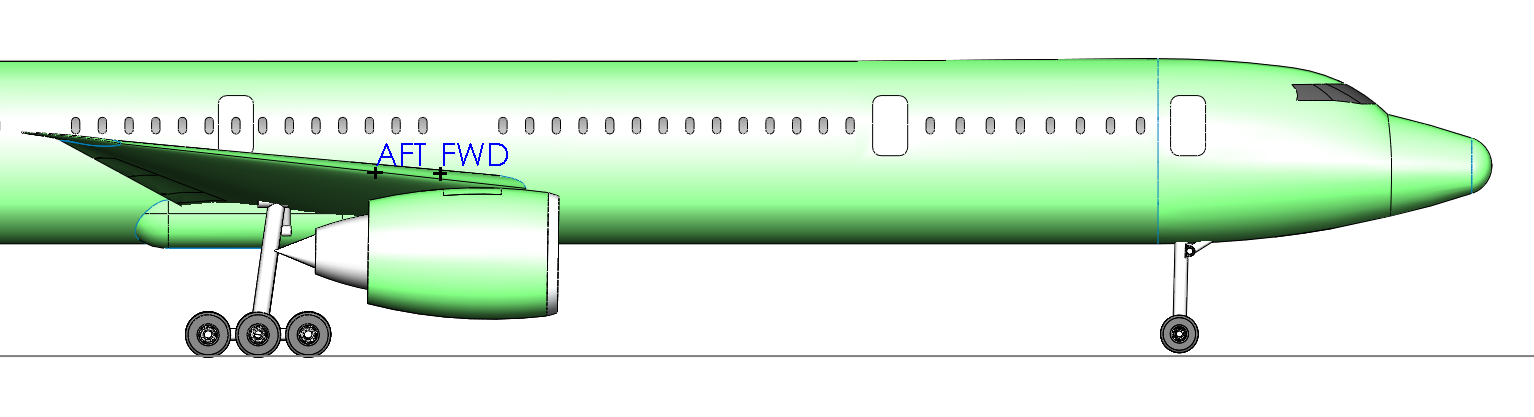
\includegraphics[width=\linewidth]{Photos/landinggear/LG Close Side View with CG.PNG}
    \caption{SAM Mk1 Landing Gear in Relation to CG Limits}
    \label{fig:landing_gear_CG}
\end{figure}


\subsubsection{Kinematics}
The landing gear must also be designed in such a way which allows seamless stowage into the belly of the aircraft. In Figs. \ref{fig:main_landing_kin} and \ref{fig:nose_landing_kin}, the kinematics of the main and nose landing gear are shown. As seen, both the main and nose landing gear stow into the aircraft without interference.

\begin{figure}[!h]
    \centering
    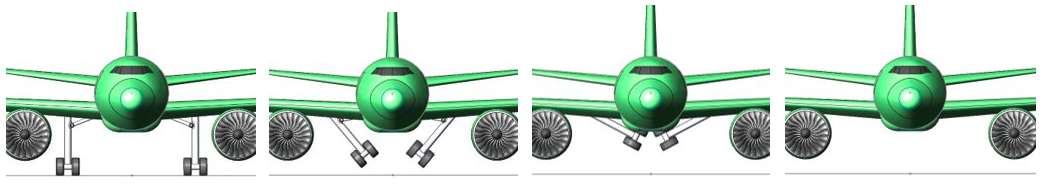
\includegraphics[width=\linewidth]{Photos/landinggear/Main Gear Kinematics.PNG}
    \caption{SAM Mk. I Main Landing Gear Kinematics}
    \label{fig:main_landing_kin}
\end{figure}

\begin{figure}[!h]
    \centering
    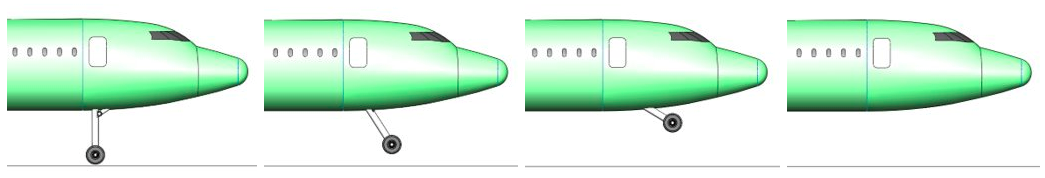
\includegraphics[width=\linewidth]{Photos/landinggear/Nose Gear Kinematics.PNG}
    \caption{SAM Mk. I Nose Landing Gear Kinematics}
    \label{fig:nose_landing_kin}
\end{figure}


\subsubsection{Tire Selection (JJ)}
With the SAM Mark I falling within the weight and size boundaries of established commercial aircraft, designing to utilize tires already available from known manufacturers saves cost and time, and also mitigates the threat of setbacks due to developmental overruns from the manufacturer. Bridgestone was selected as a launch supplier for both the nose (two) and main (twelve) tires using existing tires from their APR line first introduced for the Boeing 777-300ER/200LR in 2004 \cite{bridgestonetire}.  Their listed specifications, as published by Bridgestone \cite{bridgestonetire}, are below in Table \ref{tab:tires}.  Per FAA FAR Part §25.733 \cite{cfr}, the tires will be filled with dry nitrogen to mitigate issues caused by dioxygen, a powerful oxidizer, at high heats as well as moisture, both found in ambient air. 

\begin{table}[!h]
    \centering
        \caption{Tire Specifications}
    \begin{tabular}{|c||c|c|c|c|c|c|}\toprule
         & \textbf{Size} & \textbf{Ply Rating} & \textbf{Speed Rating [MPH]} & \textbf{Rated Load [lb]} & \textbf{Average Weigh [lb]} & \textbf{Model} \\\hline \hline
         \textbf{Main} & 52x21.0R22 & 36 & 235 & 66,500 & 266 & APR07700 \\ \hline
         \textbf{Nose} & 43x17.5R17 & 32 & 235 & 44,500 & 156 & APR06600 \\ \hline
    \end{tabular}
    \label{tab:tires}
\end{table}

\subsubsection{Future Work}
Future work will include a more detailed CAD model, as well as the modelling of the landing gear stowage bay. The kinematics will also be animated rather than depicted by a step-by-step collage.

% \textcolor{red}{
% \begin{itemize}
%     \item Discuss landing gear sizing, tire sizing, loads, and retraction system.
%     \item Include CAD drawings with landing gear extended and stowed.
%     \item Discuss pressurization (if used).
%     \item Consider merging into Structures as a sub section
% \end{itemize}}